\documentclass[a4paper 12pts]{article}
\usepackage[utf8]{inputenc}
\usepackage[T1]{fontenc}
\usepackage[francais]{babel}
\usepackage{graphicx}


\title{Documentation Technique : iRover}

\author{}

\begin{document}

\maketitle


\begin{figure}[h]
   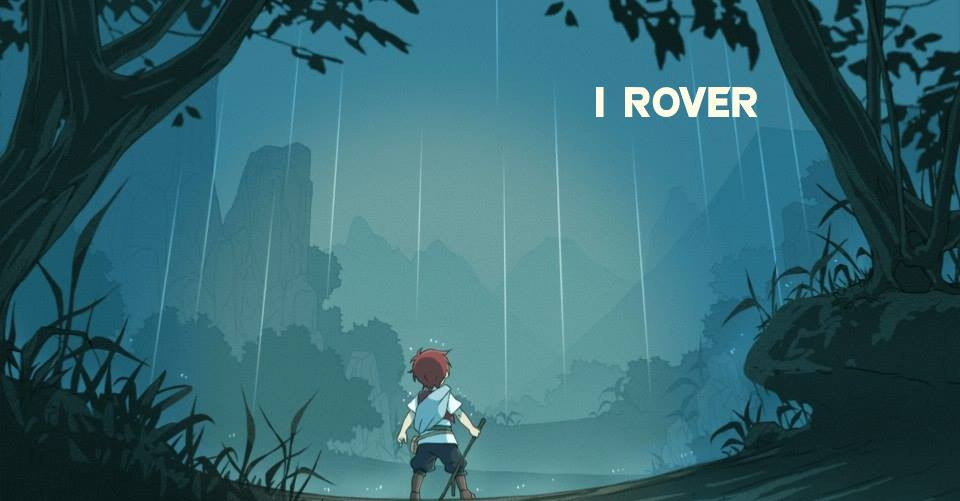
\includegraphics[width=350pt]{Illustration/proj_irover.jpg}
	\caption{iRover, l'histoire d'un héros qu'on appellait robot}
\end{figure}



\newpage


\renewcommand{\contentsname}{Sommaire} 
\tableofcontents

\newpage





\section{Manuel Documentation Technique}


\vspace{2cm}

Cette partie est dédiée aux développeurs
%expliquer à quoi sert cette documentation


\section{Les personnages}

\subsection{Le robot, Rover}

\subsection{les ennemis}



\section{les coffres}

\section{les clé}


\section{L'environnement}

Le terrain est représenté par la classe \textbf{Map}, qui contient les informations sur ce terrain (hauteur, largeur, taille des cases) et deux matrices contenant respectivement les types de cases de la carte, et la praticabilité de celles-ci. Cette dernière matrice est passée aux entités évoluant dans cette carte, pour connaître les cases passables ou non et adapter leurs algorithmes de recherche de chemin en conséquence.
Une carte se construit à partir d'un fichier au format \emph{.tmx}, un format de carte géré par le logiciel \textbf{Tiled}, un éditeur de cartes libre. Ce fichier est alors traîté comme un document DOM, grâce au module \emph{ClanXML} de la bibliothèque \emph{ClanLib 4.0}, pour en extraire les informations et les numéros des cases.
Pour gérer le dessin de la carte, la classe \textbf{Tileset} permet de représenter une feuille de textures consistant en une image regroupant toutes les textures des cases pouvant être dessinées. Ce tileset possède des métadonnées telles que le nombre de textures en lignes, colonnes, leur taille en pixels et l'espacement entre chacun dans l'image, métadonnées qui peut être récupérées également depuis le fichier de carte .tmx fourni. A partir d'un numéro de tile à une certaine position dans la carte, on peut alors déterminer quelle texture doit être dessinée à l'emplacement correspondant. 
La classe \textbf{mapDisplay} est pour l'instant la classe principale de l'application, où sont affichés la carte et tous les éléments interagissant avec. Tout l'affichage est géré par le module \emph{ClanDisplay} de la bibliothèque \emph{ClanLib 4.0}, qui dessine au milieu de la fenêtre toute la carte case par case conformément au Tileset fourni, ainsi que tous les personnages et les objets.

\section{La gestion des évênements}


\subsection {Rencontre avec un ennemi} 
\subsection {Ouvertude d'un coffre}
\subsection {Ramasser une clé}


\section{l'interface utilisateur}

\section{IA}

\subsection{path finding}

\subsection{découverte de la carte}

\section{condition fin de jeu}

\section {FAQ}




\end{document}

